% !TeX program = tectonic
\documentclass[10pt,aspectratio=169]{virgiling-slides}

\usepackage{mathtools}
\usepackage{booktabs}
\usepackage{tikz}
\usepackage[
  backend=bibtex,
  style=alphabetic,
  sorting=none,
  giveninits=true,
  maxalphanames=3,
  minalphanames=3,
  maxbibnames=3,
  minbibnames=3,
  doi=false,
  isbn=false,
  url=false,
  eprint=false
]{biblatex}
\usetikzlibrary{arrows.meta,positioning}
\addbibresource{references.bib}
\DeclareFieldFormat[inproceedings]{booktitle}{\textcolor{black!55}{\mkbibemph{#1}}}

% Short values in brackets are used in the footer.
\title[Presentation Title]{A Complete Example Presentation}
\subtitle{A feature tour of virgiling-slides}
\author[Your Name]{Your Name}
\institute[Your Institution]{Your Department or Research Group\\Your Institution}
% The class defaults to the compilation date and current year.
% \date[Event \quad 2026]{Event or Seminar Name\\Month 2026}

% Optional features:
% \titlegraphic{\includegraphics[height=8mm]{figures/logo.pdf}}
% \VirgilingEnableSectionOutlines[Section Overview]
% \setbeameroption{show notes}

% Optional footer overrides:
% \renewcommand{\VirgilingFooterLeft}{Your Name (Institution)}
% \renewcommand{\VirgilingFooterCenter}{Short Presentation Title}
% \renewcommand{\VirgilingFooterRight}{Event 2026\hfill\insertframenumber/\inserttotalframenumber}

\begin{document}

\VirgilingTitleFrame

\begingroup
  \setcounter{tocdepth}{1}
  \VirgilingOutlineFrame[Presentation Overview]
\endgroup

\section{Essentials}

\subsection{Frame Anatomy}

\begin{frame}{Frame Title}
  \framesubtitle{An optional subtitle for context}

  Ordinary frames are top-aligned. Keep one primary message on each slide and
  use the short metadata forms to keep the footer compact.

  \bigskip
  \begin{description}
    \item[Structure] Use \texttt{section} and \texttt{subsection} to populate the top navigation.
    \item[Emphasis] Combine \structure{structural emphasis}, \alert{important cautions}, and \emph{local stress} sparingly.
    \item[Alignment] Add the \texttt{[c]} frame option when vertically centered content is more appropriate.
  \end{description}

  \note{Speaker notes are available when the note-output option is enabled.}
\end{frame}

\subsection{Lists}

\begin{frame}{Lists and Incremental Structure}
  \begin{columns}[T,onlytextwidth]
    \begin{column}{0.47\textwidth}
      \textbf{Unordered list}
      \begin{itemize}
        \item State the main point first.
        \item Group related evidence.
          \begin{itemize}
            \item Nested items remain visually subordinate.
            \item Square markers are used consistently.
          \end{itemize}
        \item End with the implication.
      \end{itemize}
    \end{column}
    \begin{column}{0.47\textwidth}
      \textbf{Ordered list}
      \begin{enumerate}
        \item Introduce the input.
        \item Explain the operation.
        \item Present the result.
      \end{enumerate}
    \end{column}
  \end{columns}
\end{frame}

\subsection{Columns and Blocks}

\begin{frame}{Columns and Semantic Blocks}
  \begin{columns}[T,onlytextwidth]
    \begin{column}{0.48\textwidth}
      \begin{block}{Standard block}
        Use for definitions, context, or the main argument.
      \end{block}

      \begin{exampleblock}{Example block}
        Use for validated results, opportunities, or positive outcomes.
      \end{exampleblock}
    \end{column}
    \begin{column}{0.48\textwidth}
      \begin{alertblock}{Alert block}
        Reserve this treatment for assumptions, limitations, or risks.
      \end{alertblock}

      \begin{block}{Layout rule}
        Prefer balanced column widths and align columns at the top with
        \texttt{[T,onlytextwidth]}.
      \end{block}
    \end{column}
  \end{columns}
\end{frame}

\section{Visuals}

\subsection{Mathematics}

\begin{frame}{Mathematical Typesetting}
  Inline mathematics uses Cambria Math, for example
  $f\colon \mathbb{R}^n \to \mathbb{R}$ and $\nabla f(x^\star)=0$.

  \begin{columns}[T,onlytextwidth]
    \begin{column}{0.48\textwidth}
      \begin{align*}
        p(y\mid x)
          &= \frac{p(x\mid y)p(y)}{p(x)}, \\
        \widehat{\theta}
          &= \arg\min_{\theta}\sum_{i=1}^{m}
             \lVert y_i-g_{\theta}(x_i)\rVert_2^2.
      \end{align*}
    \end{column}
    \begin{column}{0.48\textwidth}
      \[
        h(t)=
        \begin{cases}
          0, & t < 0,\\
          t^2, & 0 \leq t < 1,\\
          1, & t \geq 1.
        \end{cases}
      \]
    \end{column}
  \end{columns}

  \begin{block}{Tip}
    Use display equations only when the notation is part of the slide's main message.
  \end{block}
\end{frame}

\subsection{Theorems}

\begin{frame}{Theorems, Definitions, and Proofs}
  \begin{definition}[Stable update]
    An update rule $T$ is stable on $D$ if
    $\lVert T(x)-T(y)\rVert \leq \lVert x-y\rVert$ for all $x,y\in D$.
  \end{definition}

  \begin{theorem}[Sample result]
    If $T$ is a contraction on a complete metric space, then $T$ has a unique
    fixed point.
  \end{theorem}

  \begin{proof}
    Iterating $x_{k+1}=T(x_k)$ gives a Cauchy sequence; completeness provides a
    limit, and contraction gives uniqueness.
  \end{proof}
\end{frame}

\subsection{Tables}

\begin{frame}{Tables for Compact Comparisons}
  \begin{table}
    \centering
    \caption{Use direct labels, aligned precision, and minimal rules.}
    \begin{tabular}{@{}lrrr@{}}
      \toprule
      Method & Accuracy & Time (s) & Memory (GB) \\
      \midrule
      Baseline & 82.4 & 18.7 & 3.8 \\
      Variant A & 85.1 & 14.2 & 3.1 \\
      Variant B & \textbf{87.6} & \textbf{11.9} & 3.3 \\
      \bottomrule
    \end{tabular}
  \end{table}

  \begin{exampleblock}{Takeaway}
    Put the interpretation below the table instead of asking the audience to
    infer the important comparison on their own.
  \end{exampleblock}
\end{frame}

\subsection{Figures}

\begin{frame}{Self-Contained Diagrams and External Figures}
  \begin{figure}
    \centering
    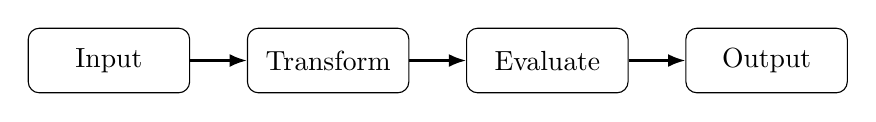
\begin{tikzpicture}[
      node distance=0.72cm,
      stage/.style={draw,rounded corners,minimum width=2.05cm,minimum height=0.82cm,align=center},
      flow/.style={-{Latex[length=2.2mm]},thick}
    ]
      \node[stage] (input) {Input};
      \node[stage,right=of input] (transform) {Transform};
      \node[stage,right=of transform] (evaluate) {Evaluate};
      \node[stage,right=of evaluate] (output) {Output};
      \draw[flow] (input) -- (transform);
      \draw[flow] (transform) -- (evaluate);
      \draw[flow] (evaluate) -- (output);
    \end{tikzpicture}
    \caption{TikZ keeps simple diagrams sharp at every projection size.}
  \end{figure}

  For an external vector figure, use for example:
  \begin{center}
    \texttt{\textbackslash includegraphics[width=.82\textbackslash linewidth]\{figures/result.pdf\}}
  \end{center}
\end{frame}

\section{Delivery}

\subsection{Code}

\begin{frame}[fragile]{Code and Monospace Text}
  \begin{columns}[T,onlytextwidth]
    \begin{column}{0.59\textwidth}
\begin{lstlisting}[language=Python,numbers=left]
def normalize(values):
    # Return a normalized copy.
    if not values:
        raise ValueError("empty input")
    total = sum(values)
    return [value / total for value in values]
\end{lstlisting}
    \end{column}
    \begin{column}{0.36\textwidth}
      The \texttt{virgiling} listings style provides:
      \begin{itemize}
        \item language-aware syntax colors;
        \item optional line numbers;
        \item automatic line wrapping;
        \item MD IO throughout.
      \end{itemize}
    \end{column}
  \end{columns}

  \medskip
  \texttt{tectonic -X compile talk.tex --synctex}
\end{frame}

\subsection{Overlays}

\begin{frame}{Purposeful Overlays}
  \begin{enumerate}[<+->]
    \item Reveal the question before the answer.
    \item Add evidence in the order it will be discussed.
    \item Leave the final slide state complete and understandable.
  \end{enumerate}

  \uncover<3->{
    \begin{block}{Handout mode}
      Add the \texttt{handout} class option to collapse overlays when preparing
      a printable version.
    \end{block}
  }
\end{frame}

\subsection{Navigation}

\begin{frame}{Links, Footnotes, and Navigation}
  \hypertarget{navigation-demo}{}

  Standard Beamer and Hyperref commands remain available:
  \begin{itemize}
    \item External link: \href{https://ctan.org/pkg/beamer}{Beamer on CTAN}.
    \item Alphabetic citations: one author gives \cite{lamport1994latex}; a larger team gives \cite{vaswani2017attention}.
    \item Footnote: use footnotes for qualifications that should remain visible.\footnote{Keep footnotes short enough to read during the talk.}
    \item Internal navigation: jump to supporting material without changing the main flow.
  \end{itemize}

  \begin{center}
    \hyperlink{backup-demo}{\beamergotobutton{Jump to backup slide}}
  \end{center}
\end{frame}

\subsection{Closing}

\begin{frame}[c]{Questions?}
  \begin{center}
    \Large Thank you\\[0.8em]
    \normalsize
    Your Name\\
    \texttt{you@example.com}

    \bigskip
    \structure{Project, paper, or profile URL}
  \end{center}
\end{frame}

\appendix
\section{Appendix}

\subsection{Backup}

\begin{frame}{Backup Material}
  \hypertarget{backup-demo}{}

  Backup slides can contain:
  \begin{itemize}
    \item additional derivations or implementation details;
    \item robustness checks and extended tables;
    \item answers to likely audience questions.
  \end{itemize}

  \begin{block}{Main-deck discipline}
    Move useful but nonessential detail here so the primary narrative stays focused.
  \end{block}

  \begin{center}
    \hyperlink{navigation-demo}{\beamerreturnbutton{Return to navigation example}}
  \end{center}
\end{frame}

\subsection{References}

\begin{frame}{References}
  \printbibliography[heading=none]
\end{frame}

\end{document}
